\section{Latent Ordinary and Stochastic Differential Equations models : a trailer}\label{Latent Ordinary and Stochastic Differential Equations models}

\begin{frame}{Latent ODE}
    \begin{itemize}
        \item \glspl{latent ode} is a class of models introduced in \cite{chen_neural_2019} : "Neural Ordinary Differential Equations" 
by Ricky T. Q. Chen, Yulia Rubanova, Jesse Bettencourt, David Duvenaud. 
ArXiV : \href{https://arxiv.org/abs/1806.07366}{Neural ODE Best Paper Award NeurIPS 2018}.
        \item Starting point : assume ResNet-like evolution of latent
            \begin{align}
                z_{t+1} &= z_t + f(z_t, \theta_t)
            \end{align}
        \item becomes in continuous time:
        \begin{align}
                \frac{dz_t}{dt} &= f(z_t, t, \theta_f)
        \end{align}
            where $\theta_f$ is a set of parameters, that can typically be the parameters of 
            a neural network learning $f$.
    \end{itemize}
\end{frame}

\begin{frame}{Latent ODE - model}
    \begin{itemize}
        \item Generative model
            \begin{align}
                z_{t_0} &\sim p_{\theta_z}(z_{t_0}) \\
                z_{t_1}, z_{t_2}, ..., z_{t_N} &= \text{ODE Solver}(z_{t_0}, f, \theta_f, t_0, ..., t_N ) \\
                x_{t_i} &\sim p_{\theta_x}(x_t \vert z_t)
            \end{align}
        \item Inference
        \begin{align}
                [\mu_\phi, \Sigma_\phi] &= \text{LSTM} (x_{t_0:t_N})   \\
                q_{\phi}(z_{t_0} \vert x_{t_0:t_N}) &= \mathcal{N}(z_{t_0} \vert \mu_{\phi}, \Sigma_\phi)
        \end{align}
    \end{itemize}
\end{frame}

\begin{frame}{Latent ODE - model}
    We reproduce here the drawing from the paper:
    \begin{figure}[H]
        \centering
        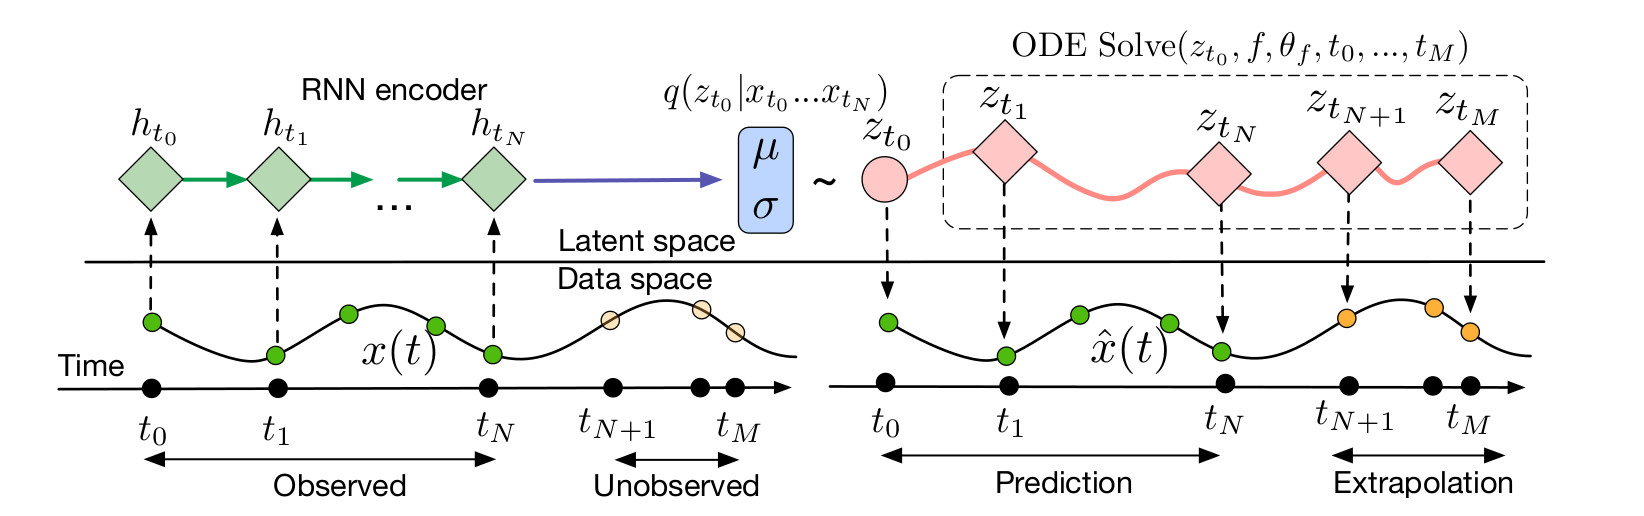
\includegraphics[width=0.9\textwidth]{/home/benjamin/Folders_Python/MVA/MVA_Stage/images/Neural_ODE_01.png}
        \caption{Neural ODE model}
        \label{fig:Neural ODE}
    \end{figure}
\end{frame}

\begin{frame}{Latent ODE - ELBO}
    \begin{itemize}
        \item the stochastic variables are $z_{t_0}$ and the $x_{t_i}$'s.
        \item the joint distribution writes:
            \begin{align}
                p(x_{t_1:t_N}, z_{t_0}) 
                % &= p(z_{t_0})p(x_{t_1:t_N} \vert z_{t_0}) \\
                &= p(z_{t_0}) \prod_{t=1}^{N}p_{\theta_x}(x_{t_i} \vert z_{t_i})
            \end{align}
        \item likelihood:
        \begin{align}
            % p(x_{t_1:t_N}) &= \frac{p(x_{t_1:t_N}, z_{t_0})}{p(z_{t_0} \vert x_{t_1:t_N})} \\
            \log{p(x_{t_1:t_N})} 
            % &= \mathbb{E}_{q_{\phi}(z_{t_0} \vert x_{t_1:t_N})} \log{\frac{p(x_{t_1:t_N}, z_{t_0})}{q_{\phi}(z_{t_0}\vert x_{t_1:t_N})}\frac{q_{\phi}(z_{t_0}\vert x_{t_1:t_N})}{p(z_{t_0} \vert x_{t_1:t_N})}} \\
            % \log{p(x_{t_1:t_N})} 
            &\geq \mathbb{E}_{q_{\phi}(z_{t_0} \vert x_{t_1:t_N})} \log{\frac{p(x_{t_1:t_N}, z_{t_0})}{q_{\phi}(z_{t_0}\vert x_{t_1:t_N})}} \\
                % &= \mathbb{E}_{q_{\phi}(z_{t_0} \vert x_{t_1:t_N})} \log{\frac{p(z_{t_0}) \prod_{t=1}^{N}p_{\theta_x}(x_{t_i} \vert z_{t_i})}{q_{\phi}(z_{t_0}\vert x_{t_1:t_N})}} \\
                &= \sum_{i=1}^{N} \mathbb{E}_{q_{\phi}(z_{t_0} \vert x_{t_1:t_N})} \log{p_{\theta_x}(x_{t_i} \vert z_{t_i})} - \mathbb{KL}(q_{\phi}(z_{t_0} \vert x_{t_1:t_N}) \vert\vert p(z_{t_0}))
        \end{align}
        \item Need to compute the gradients of $\log{p_{\theta_x}(x_{t_i} \vert z_{t_i})}$ w.r.t. $\theta_f$. 
        Methods are forward sensivity, backpropragation through \gls{ode} solver, or \textbf{adjoint sensitivity method}.
        (see \cite{pontriagin_mathematical_2018}, \cite{sengupta_efficient_2014}).
        % \ref{sec:adjoint_sensitivity_method}.
    \end{itemize}
\end{frame}

% A limitation of this model is the assumption that the prior is "concentrated" in the initial value $z_{t_0}$, and that the 
% remaining latent variables are deterministically determined.
% \end{frame}

\begin{frame}{Latent SDE Model}
    \glspl{latent ode} models have limitations :
        \begin{itemize}
            \item the latent dynamic is deterministic by design
            \item the intial variable $z_{t_0}$ encompasses the entire randomness of the prior, and can become
            unnaturally large to account for randomness along the entire timeline
        \end{itemize}

    The idea in \cite{li_scalable_2020} is to add some noise to the deterministic computation of the latent variable:
        \begin{align}
            \frac{dz_t}{dt} &= f_{\theta_f}(z_t,t) + \epsilon_t \\
            \epsilon_t &\sim \mathcal{N}(0,Q \textit{Id})
        \end{align}
    Which leads to an \gls{sde} prior:
        \begin{align}
            \label{latent sde prior}
            dZ_t &= f_{\theta}(Z_t, t)dt + \sigma_{\theta}(Z_t,t)dB_t \\
            Z_{t_0} &\sim Z_0
        \end{align}
    (where we used $\sigma_{\theta}$ instead of our usual $L(Z_t,t)$ to stick to the notations of the paper).

    \ref{latent sde prior} defines a prior distribution over functions. In order to draw a sample function, we would:
        \begin{itemize}
            \item draw a sample $z_{t_0} \sim Z_0$
            \item draw a random Brownian motion $\tilde{B_t}$ path from $B_t$
            \item compute $z_t - z_{t_0} = \int_{t_0}^{t} f_{\theta}(Z_t, t)dt + \int_{t_0}^{t} \sigma_{\theta}(Z_t,t)d\tilde{B_t}$
        \end{itemize}
\end{frame}

\begin{frame}{Latent SDE - generative model}
    The approximate posterior can also be described as a \gls{sde}:
        \begin{align}
            dZ_t &= f_{\phi}(Z_t,t)dt + \sigma_{\phi \, = \, \theta}(Z_t,t)dB_t \\
            Z_{t_0} &= z_0 \, \text{from prior}
        \end{align}
        \begin{itemize}
            \item the prior and the approximate posterior share the same diffusion for the $\mathbb{KL}$ to have the same support
            \item the prior and the approximate posterior have the same starting value $z_0$
        \end{itemize}
    \begin{figure}[H]
        \centering
        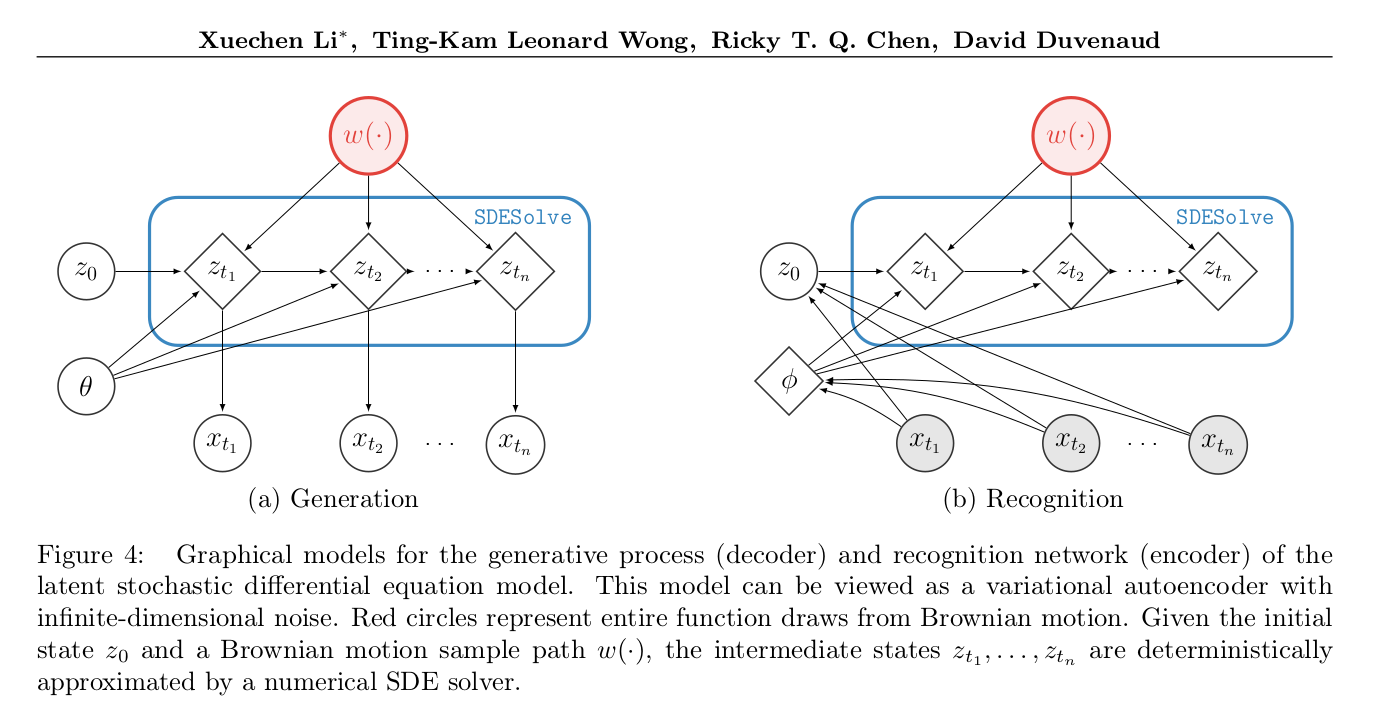
\includegraphics[width=0.7\textwidth]{/home/benjamin/Folders_Python/MVA/MVA_Stage/images/Latent_SDE_01.png}
        \caption{Latent SDE model}
        \label{fig:Latent SDE}
    \end{figure}
\end{frame}

\begin{frame}{Latent SDE - inference}
    \begin{itemize}
        \item neural networks to learn the drift $f_{\phi}$ and the diffusion $\sigma_{\theta}$
        \item requires to compute the gradient of functionals (loss) of type:
            \begin{align}
                L(\theta, \phi) &= L \left( \int_{t_0}^{t_1} f_{\phi}(Z_t, t)dt + \int_{t_0}^{t} \sigma_{\theta}(Z_t,t)dB_t \right)
            \end{align}
            where $\int_{t_0}^{t} \sigma_{\theta}(Z_t,t)dB_t$ is actually a random variable!
        \item It appears that the adjoint sensitivity method can be adapted to SDEs (see \cite{li_scalable_2020}).
    \end{itemize}
    
    The stochastic \gls{vlb} writes:
    \begin{align}
        \mathcal{L}(\theta, \phi, x_{1:T}) &= \mathbb{E} \left(
            \frac{1}{2}\int_{0}^{T} \left| \frac{f_{\theta}(z_t,t) - f_{\phi}(z_t,t)}{\sigma_{\theta}(z_t,t)} \right|^{2} dt  - 
            \sum_{i=1}^{N} \log{p_{\theta_x}}(x_{t_i} \vert z_{t_i})
            \right)
    \end{align}
\end{frame}